\subsection{Wortvorhersage}
	
    Sprachmodelle werden in einer in \autoref{fig:langugeModels} beschrieben Ordnerstrucktur gespeichert. Aus den dort angelegten Sprachmodellen werden die dem Nutzer angezeigten Kategorien generiert.
    
    \begin{figure}[H]
    		\dirtree{%
    			.1 categories.
        			.2 Sprachmodell 1.
        				.3 collocs.
        				.3 paths.
        			.2 Sprachmodell 2.
        				.3 collocs.
        				.3 paths.
        			.2 ….
			}
            \caption{Ordnerstrucktur von Sprachmodellen / Kategorien}
			\label{fig:langugeModels}
	\end{figure}
    
    Um den Ordnernamen eines Sprachmodells korrekt in der Benutzeroberfläche als Kategorie anzuzeigen, muss bei Umlauten auf die Codierung geachtet werden. Mit \autoref{code:NFC-utf8} konnte das Fehlerhafte anzeigen von Umlauten behoben werden. Nachdem z. B. der Buchstabe \texttt{ä} aus dem OS X Dateisystem gelesen wurde liegt das Zeichen als Kombination aus den zwei Teilen \texttt{a} und 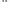
\includegraphics[]{images/dots.png} vor. Mit dem Befehl \texttt{NFC} (Normal Form Compose) kann daraus dann ein eigenes Zeichen \texttt{ä} generiert werden, welches auch in der Benutzeroberfläche korrekt angezeigt werden kann.
    
    \begin{lstlisting}[caption=Dekodierung von Ordnernamen,label=code:NFC-utf8, captionpos=b]
encoding = sys.getfilesystemencoding()
category = unicodedata.normalize("NFC", category.decode(encoding))
    \end{lstlisting}
    
    Nachdem der Nutzer eine Kategorie ausgewählt hat wird das entsprechende Sprachmodell aus den Dateien geladen. Die Dateien \texttt{collocs} und \texttt{paths} werden von dem in \autoref{sec:thirdTry} beschriebenen Programm von Liang generiert. \texttt{collocs} enthält die Übergangswahrscheinlichkeiten von einem Wort zu einem anderen. \texttt{paths} listet Worte gruppiert in Klassen zusammen mit ihrer Häufigkeit. Aus diesen Informationen können alle für die Vorhersage benötigten \emph{counts} und Wahrscheinlichkeiten berechnet werden.
    
    Die Funktion \texttt{getWordList} in der Klasse \texttt{WordPredictor} generiert eine Liste von maximal 30 Worten.
    Dazu wird für jedes Wort im Corpus die Wahrscheinlichkeit, dass dieses nach dem vorherigen Wort (oder dem Satzanfang) folgt, mit Hilfe von \autoref{eq:wordPropability} berechnet. Dann werden die Worte absteigend nach diesen Wahrscheinlichkeiten sortiert. Worte mit einer Wahrscheinlichkeit von null werden nicht zur Liste hinzugefügt. Eine optimierung dieser Rechnung, indem man beispielsweise im Voraus wie in \autoref{sec:requirements_categories} angedacht Klassen mit niedrigen Wahrscheinlichkeiten ignoriert, wird hier nicht für Nötig gehalten. Die Berechnung läuft zumindest mit den getesteten \emph{Corpi} ausreichend performant.
    
   
    
    
    
    
    
    
    
    
    
    
    
    
    
    
    
    
    
    
